\chapter{Marco Teórico}\phantom{\cite{beetz09ijcss}}

Este capítulo va a poner en contexto al lector con respecto a conceptos básicos de criptografía para posteriormente explicar los algoritmos que van a ser implementados en el FPGA.

\subsection{Conceptos Básicos}
Según la Real Academia Española la criptografía se define como 

\emph{Arte de escribir con clave secreta o de un modo enigmático.}


El mensaje que se desea transmitir es usualmente llamado \textit{texto plano} o simplemente \textit{mensaje}. Este mensaje pasa por un proceso donde se disfraza el texto plano en un \textit{texto cifrado}, este proceso es llamado \textit{cifrado}. El proceso inverso donde se toma un texto cifrado en un texto plano se llama \textit{descifrado} ambos procesos son controlados por una \textit{llave} la cual indica 



\begin{figure}
	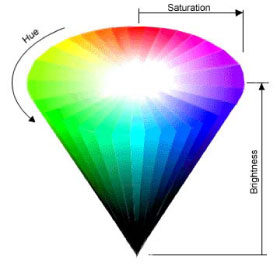
\includegraphics[width=0.4\linewidth]{images/hsb}
	\caption{Espacio de color HSI} \label{fig:hsb}
\end{figure}
\begin{figure}
	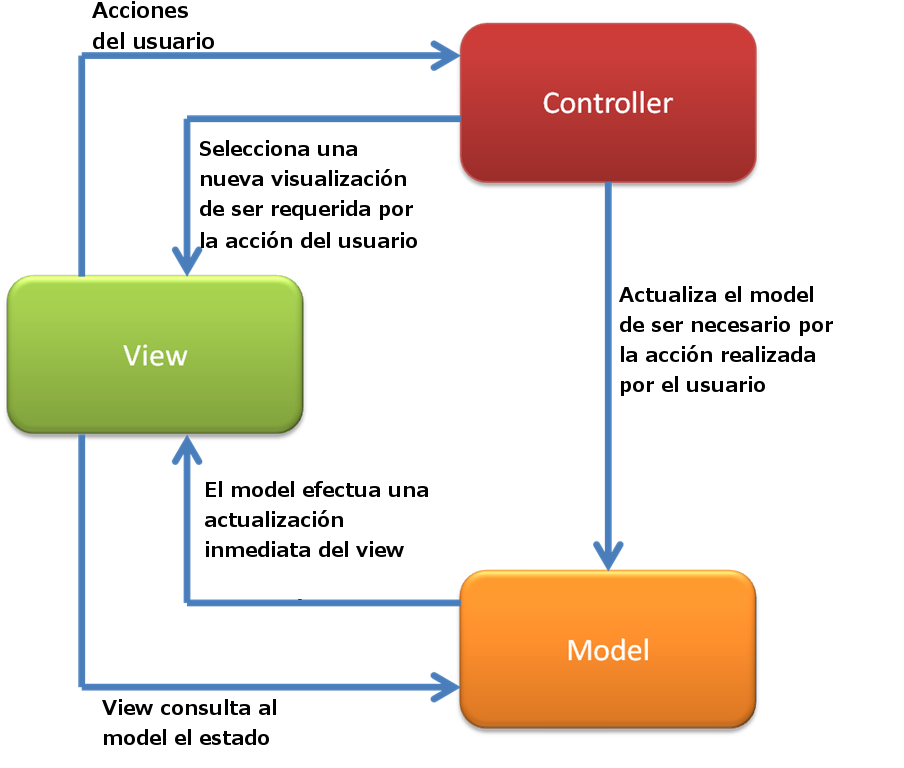
\includegraphics[width=1\linewidth]{images/mvcbase}
	\caption{Patrón de diseño MVC} \label{fig:mvc}
\end{figure}

